\documentclass[runningheads]{llncs}
\usepackage{amsmath}
\usepackage{amssymb}
\usepackage{booktabs}
\usepackage{color}
\usepackage[T1]{fontenc}
\usepackage[utf8]{inputenc}
\usepackage{graphicx}
\usepackage[bookmarksdepth=2]{hyperref}
\usepackage{listings}
\usepackage{tikz}
\usetikzlibrary{arrows.meta,positioning,fit,backgrounds}
\usepackage{xspace}
\usepackage{multirow}

\let\llncssubparagraph\subparagraph
\let\subparagraph\paragraph
\usepackage[compact]{titlesec}
\let\subparagraph\llncssubparagraph
\titlespacing*{\section}{0pt}{*2.0}{*2.0}
\titlespacing*{\subsection}{0pt}{*1.5}{*1.0}
\titlespacing*{\subsubsection}{0pt}{*0.6}{*0.4}
\setlength{\parskip}{0pt}
\setlength{\parindent}{10pt}

\definecolor{keywordcolor}{rgb}{0.7, 0.1, 0.1}
\definecolor{tacticcolor}{rgb}{0.0, 0.1, 0.6}
\definecolor{commentcolor}{rgb}{0.4, 0.4, 0.4}
\definecolor{symbolcolor}{rgb}{0.0, 0.1, 0.6}
\definecolor{sortcolor}{rgb}{0.1, 0.5, 0.1}
\definecolor{attributecolor}{rgb}{0.7, 0.1, 0.1}
\lstloadlanguages{LISP}
\def\lstlanguagefiles{lstlean.tex}
\lstset{language=lean}
\lstset{extendedchars=true,inputencoding=utf8,basicstyle=\ttfamily\small}

\DeclareUnicodeCharacter{03B1}{$\alpha$}
\DeclareUnicodeCharacter{0393}{$\Gamma$}
\DeclareUnicodeCharacter{2200}{$\forall$}
\DeclareUnicodeCharacter{2203}{$\exists$}
\DeclareUnicodeCharacter{2227}{$\wedge$}
\DeclareUnicodeCharacter{2228}{$\vee$}
\DeclareUnicodeCharacter{00AC}{$\neg$}
\DeclareUnicodeCharacter{2192}{$\rightarrow$}
\DeclareUnicodeCharacter{2194}{$\leftrightarrow$}
\DeclareUnicodeCharacter{2026}{\ldots}
\DeclareUnicodeCharacter{21A6}{$\mapsto$}
\DeclareUnicodeCharacter{2260}{$\neq$}
\DeclareUnicodeCharacter{2264}{$\le$}
\DeclareUnicodeCharacter{2208}{$\in$}
\DeclareUnicodeCharacter{2081}{$_{1}$}
\DeclareUnicodeCharacter{2082}{$_{2}$}
\DeclareUnicodeCharacter{2099}{$_{n}$}
\DeclareUnicodeCharacter{1D62}{$_{i}$}
\DeclareUnicodeCharacter{25B7}{$\triangleright$}
\DeclareUnicodeCharacter{2243}{$\simeq$}
\DeclareUnicodeCharacter{2261}{$\equiv$}
\DeclareUnicodeCharacter{2218}{$\circ$}
\DeclareUnicodeCharacter{22A4}{$\top$}
\DeclareUnicodeCharacter{22A5}{$\bot$}

\hypersetup{pdfborder={0 0 0}, colorlinks=true, linkcolor=gray, urlcolor=gray, citecolor=gray}
\renewcommand\UrlFont{\color{blue}\rmfamily}
\setlength{\textfloatsep}{10pt plus 1.0pt minus 2.0pt}

\newcommand{\cvcv}{\textsc{cvc5}\xspace}
\newcommand{\tactic}{\textsc{lean-smt}\xspace}
\newcommand{\carcara}{\textsc{Carcara}\xspace}
\newcommand{\verit}{\textsc{veriT}\xspace}
\newcommand{\alethe}{Alethe\xspace}
\newcommand{\cpc}{CPC\xspace}
\newcommand{\rare}{RARE\xspace}
\newcommand{\rulename}[1]{\texttt{#1}}
\newcommand{\subst}{\ensuremath{\mathit{subst}}}

\title{Checking \alethe Proofs with \tactic}
\titlerunning{Checking Alethe Proofs with Lean-SMT}
\author{A summary of the work on the \texttt{alethe} branch of \tactic}
\authorrunning{Alethe proofs in Lean-SMT}
\institute{Universidade Federal de Minas Gerais, Belo Horizonte, Brazil}

\begin{document}
\maketitle

\begin{abstract}
  \tactic~\cite{Mohamed2025} reconstructs \cvcv's \cpc proofs into Lean proofs,
  driving the solver through its API. This note describes an extension that checks textual
  \alethe proofs, as produced by \cvcv and \verit and elaborated by \carcara,
  against SMT-LIB problems, reusing \tactic's term reconstruction, lemma
  libraries, and arithmetic decision procedures. We describe the pipeline, how
  \alethe's contexts and clauses are handled, how the proof rules are
  reconstructed, and how the proof reaches the kernel: step by step, in
  batches, or as one term. We close with the state of the evaluation and what
  it revealed about the proofs themselves.
\end{abstract}

\section{System Overview}
\label{sec:overview}

Figure~\ref{fig:arch} depicts the pipeline. The input is an SMT-LIB problem
and an \alethe proof of its unsatisfiability, produced by \cvcv
(\texttt{-{}-proof-format-mode=alethe}) or by \verit. The proof first goes
through \carcara's~\cite{Andreotti2023} \emph{elaborator}, which turns the coarse rules of the
solver output into steps the checker can replay: the \texttt{polyeq} pass
removes the polyequalities and implicit contexts of \rulename{assume},
\rulename{refl} and \rulename{forall\_inst}; the \texttt{local} pass
canonicalizes \rulename{trans}, \rulename{cong} and resolution, writing the
pivots as arguments; and the \texttt{core} pass reduces the rules we chose
not to reconstruct in Lean to rules we do reconstruct, restricted to a list
given on the command line. The elaborated proof is then read by \tactic. Its
\emph{parser} eliminates the binding constructs of the text, its
\emph{realizer} hands every term to \cvcv's own parser through the Lean API,
so that the reconstruction of terms is the one \tactic already has for \cpc
proofs, and its \emph{reconstructor} replays the proof rule by rule, sending
each step to Lean's kernel as it goes. The verdict distinguishes a
\emph{valid} proof, in which every step was reconstructed and accepted by the
kernel, from a \emph{holey} one, in which some steps had to be trusted; the
trusted steps are reported by rule, and, when the checker runs as a tactic,
become goals for the user.

\begin{figure}[t]
  \centering
  \resizebox{\textwidth}{!}{%
  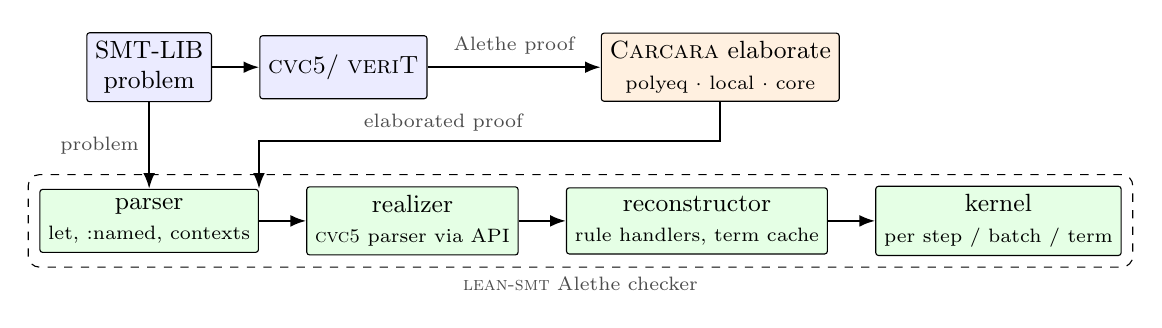
\begin{tikzpicture}[
      node distance=5mm and 6mm,
      box/.style={draw, rounded corners=1pt, align=center, font=\small, minimum height=8mm, inner sep=3pt},
      solver/.style={box, fill=blue!8},
      carc/.style={box, fill=orange!12},
      lean/.style={box, fill=green!10},
      arr/.style={-{Latex[length=2mm]}, thick},
      lab/.style={font=\scriptsize, text=black!70}
    ]
    \node[solver] (prob) {SMT-LIB\\problem};
    \node[solver, right=of prob] (solver) {\cvcv / \verit};
    \node[carc, right=22mm of solver] (carcara) {\carcara elaborate\\{\scriptsize polyeq $\cdot$ local $\cdot$ core}};
    \node[lean, below=11mm of prob] (parser) {parser\\{\scriptsize let, :named, contexts}};
    \node[lean, right=of parser] (realize) {realizer\\{\scriptsize \cvcv parser via API}};
    \node[lean, right=of realize] (recon) {reconstructor\\{\scriptsize rule handlers, term cache}};
    \node[lean, right=of recon] (kernel) {kernel\\{\scriptsize per step / batch / term}};
    \draw[arr] (prob) -- (solver);
    \draw[arr] (solver) -- node[above=1pt, lab] {Alethe proof} (carcara);
    \draw[arr] (carcara.south) -- ++(0,-5mm) -| node[above, lab, pos=0.3] {elaborated proof} (parser.north east);
    \draw[arr] (prob.south) -- node[left, lab] {problem} (parser.north);
    \draw[arr] (parser) -- (realize);
    \draw[arr] (realize) -- (recon);
    \draw[arr] (recon) -- (kernel);
    \begin{scope}[on background layer]
      \node[draw, dashed, rounded corners, fit=(parser)(realize)(recon)(kernel), inner sep=4pt, label={[lab]below:\tactic Alethe checker}] {};
    \end{scope}
  \end{tikzpicture}}
  \caption{Checking an \alethe proof. The solver's proof is elaborated by
    \carcara; the checker parses and realizes it with \cvcv's parser, replays
    it with \tactic's reconstruction, and submits the steps to Lean's kernel.}
  \label{fig:arch}
\end{figure}

The checker is available in three forms. The command
\lstinline{#check_alethe "P.smt2" "P.alethe"} checks a proof from files and
prints the verdict with per-phase timings; the \texttt{alethe} tactic closes
a Lean goal the way the \texttt{smt} tactic does, translating the goal,
obtaining an \alethe proof from \cvcv (in process, or from an external
binary), running \carcara, and reconstructing the result as a proof term of
the goal; and the underlying \texttt{checkAlethe} function serves an
executable for batch evaluation. The trusted computing base is the one of
\cpc reconstruction: Lean's kernel, and \cvcv's parser for the statement.

The rest of this section follows the pipeline: the treatment of the proof
text (Section~\ref{sec:parsing}), the replay of steps and their submission
to the kernel (Section~\ref{sec:steps}), the reconstruction techniques per
rule (Section~\ref{sec:rules}), and the changes this required in \carcara
(Section~\ref{sec:carcara}). Section~\ref{sec:eval} reports the evaluation,
Section~\ref{sec:shapes} the comparison of the kernel submission shapes, and
Section~\ref{sec:native} that of the \texttt{native} variant against the
kernel-checked default.

\subsection{From Proof Text to Terms}
\label{sec:parsing}

\paragraph{Binding constructs.} An \alethe proof, as \carcara prints it,
shares subterms with \texttt{(! t :named @p\_n)} annotations and, in \verit's
case, with \texttt{let}. The parser eliminates both over a hash-consed arena
of S-expressions, so that substitution never copies a term: a \texttt{let}
is a scoped parallel binding, and a name stands for the annotated term from
its definition onward. Anchor variables, the \texttt{(x S)} and
\texttt{(:= x t)} arguments of an \texttt{anchor} command, are renamed to
globally fresh symbols inside their block. The realizer then serializes each
literal once, binding every shared subterm on first use as a fresh constant
\texttt{s\textasciitilde{}n}, so that \cvcv's hash-consing and \tactic's term
cache keep the Lean terms shared as well.

\paragraph{Contexts.} \alethe's subproofs under an anchor with
\texttt{(:= x t)} arguments carry a context $\Gamma$, and a step
$\Gamma \triangleright s \simeq u$ inside it means $\subst(\Gamma)(s) = u$: the
substitution applies to the left-hand side only, and
$\subst(\Gamma, x \mapsto t) = \subst(\Gamma) \circ \{x \mapsto t\}$, as in
the semantics of Barbosa et al.\ for formula processing~\cite{Barbosa2020}
and in \carcara. The checker encodes an assignment as a \texttt{let}-bound
local, so that inside the block the replaced variable unfolds to its value
definitionally, and the bind rules read the substitution off that unfolding.
To give the two sides of a judgment their two meanings, the parser carries
two environments per context, the \emph{substituted} one (with the
renamings) and the \emph{fixed} one (the enclosing environment plus the
context's own variables), and parses a unit clause \texttt{(= l r)} with
\texttt{l} under the first and \texttt{r} under the second. Where no
substitution is in scope the two coincide. This is what makes \verit's
nested renamings checkable, where an inner \rulename{bind} replaces a name
that the enclosing \rulename{bind} had just introduced as a fixed variable; such proofs are valid under the paper's calculus but outside the canonical
fragment its algorithm produces, and were previously unrepresentable.

The same machinery absorbs a quirk of \verit's sharing: with
\texttt{-{}-proof-with-sharing}, \verit names terms that are \emph{open} in
let-bound variables and reuses the names under other bindings of those
variables. Read as SMT-LIB, where a name denotes the closed term at its
definition, most of \verit's QF\_UF proofs state assumptions that are not the
problem's assertions. Read as macros over the let-bound variables they
mention, they do. Both \carcara and the checker now resolve a name anew in
every scope it is used in, closed names being unaffected.

\paragraph{Realization.} Terms are realized by \cvcv's parser in the
higher-order logic \texttt{HO\_ALL}, so that a \texttt{choice} binder can be
represented as a per-sort constant applied to a \texttt{lambda} and later
mapped to \texttt{Classical.epsilon}. Integer numerals in real-only logics
are read as reals, as both solvers do. From this point on, the reconstruction
of sorts and terms is \tactic's \texttt{reconstructTerm}, unchanged.

\subsection{Replaying Steps and Reaching the Kernel}
\label{sec:steps}

\paragraph{Steps and clauses.} A step is handed to the rule reconstructors
as a record of its clause literals, rule, premises (with their literals and
the Lean proof of their clause), arguments, discharged assumptions, and,
for the closing step of a subproof, the anchor's variables, assignments and
last step. Reconstructors are registered with an attribute,
\lstinline{@[alethe_rule_reconstruct]}, one per theory, and dispatch on the
rule name. A clause \texttt{(cl l₁ …\ lₙ)} is the right-nested disjunction
of its literals, definitionally \lstinline{orN [l₁, ..., lₙ]}, so that the
\lstinline{orN} lemmas of \tactic apply. \alethe's clauses are sets, and
elaborated resolutions state their conclusions modulo permutation and
duplicate removal, so a computed clause is aligned with the stated one by
\lstinline{orN_of_map}: an index map from the stated literals to the computed
ones, checked by the kernel by evaluation, proves the stated clause from the
computed one; the associative-commutative rewriting of \texttt{ac\_rfl} is
kept only as a fallback.

\paragraph{Step by step.} \cpc reconstruction in \tactic builds one proof
term for the whole proof and submits it to the kernel once. The \alethe
checker instead checks every top-level step on its own: the step's proof is
type-checked by \texttt{Kernel.check} against its stated clause in a local
context holding the problem's symbols and assertions and only the earlier
steps the proof mentions, as hypotheses; the proof term is then dropped and
the step becomes a hypothesis for the steps after it. Steps inside a
subproof are kept as terms, since the closing step's proof abstracts over
the block's assumptions and variables, and are checked with it. Memory stays
bounded by the largest step rather than the whole proof, a failure is
attributed to the step the kernel rejected, and the checked count is exact.
The cost is that every kernel call starts with an empty inference cache.

\paragraph{Batches, and one term.} Between the two extremes, consecutive
top-level steps can be gathered into one kernel call. A batch
$e_1 : c_1, \ldots, e_n : c_n$ becomes the term
\[
  (\lambda h_1 : c_1.\ (\lambda h_2 : c_2.\ \cdots (\lambda h_n : c_n.\ \mathtt{trivial})\ e_n \cdots)\ e_2)\ e_1,
\]
which the kernel accepts exactly when every $e_i$ proves $c_i$ under the
hypotheses of the steps before it: the binders keep those hypotheses opaque,
each conclusion stays an explicit annotation, and one call shares its cache
over the batch. Each proof is abstracted once over the earlier hypotheses of
its batch, so construction is linear in the batch. The batch is bounded by a
number of steps or by the number of term nodes it holds (counted with
sharing), and a rejected batch is re-checked step by step, so that what is
trusted is what the kernel actually rejected. Batches can also be dispatched
to concurrent tasks, at most a fixed number in flight, joined in step order;
the calls are independent by construction, since each establishes its
conclusions from hypotheses rather than from the earlier proofs. Finally, a
\emph{term mode} mirrors \cpc reconstruction, inlining every step into the
steps that use it and submitting one closed theorem; it is what the
\texttt{alethe} tactic uses, and the shape the evaluation compares against.

\subsection{Reconstructing the Rules}
\label{sec:rules}

The checker handles 96 \alethe rule names, in about 4\,900 lines of Lean
plus the generated \rare table, following the three techniques of \cpc
reconstruction: theorems, tactics, and verified programs. The dividing line
with \carcara is drawn per rule: a rule is reconstructed in Lean when a
direct proof is cheap and robust, and reduced by \carcara's core pass
otherwise, which the \texttt{-{}-core-rules} flag we added lets the pipeline
select rule by rule.

\paragraph{Via theorems.} The clausal rules of \alethe, the CNF axioms
(\rulename{and\_pos}, \rulename{or\_neg}, \rulename{implies\_pos},
\rulename{equiv\_neg1}, the \texttt{ite} and \texttt{xor} families) and the
elimination rules (\rulename{and}, \rulename{not\_or}, \rulename{implies},
\rulename{equiv2}, \ldots), are the \cpc lemmas of \tactic applied with the
indices \carcara's \texttt{local} pass writes as arguments. The connective
definitions, the selection axioms \rulename{ite\_then\_intro} and
\rulename{ite\_else\_intro} that the core pass derives \rulename{ite\_intro}
from, \rulename{la\_disequality}, the division rules of \cvcv
(\rulename{div\_intro}, \rulename{div\_by\_zero\_intro}) and the like are new
lemmas in an \alethe-specific library of 52 theorems.

\paragraph{Via tactics.} \rulename{la\_generic} is Farkas' lemma:
the negated literals are introduced as hypotheses, integer bounds are
tightened by the gcd of their coefficients as \carcara does (a strict bound
with unit gcd by \lstinline{Int.add_one_le_iff} alone; the rounding cases
by \texttt{omega}, given just the bound, the shape \texttt{poly\_norm}
establishes and the negated goal), the bounds are scaled by the rational
coefficients given as arguments (integer bounds cast to rationals in mixed
combinations), summed with \tactic's \texttt{sum\_ub} lemmas, normalized by
\texttt{poly\_norm}, and closed by the sign of the constant. Both details
matter at scale: a \rulename{la\_generic} with five hundred literals ran
five hundred \texttt{omega} calls over the whole local context before, and
now takes a few seconds. \rulename{cong} aligns the
premises with the argument positions, in either orientation, and falls back
to definitional equality for arguments that differ only by the context's
substitutions or by \texttt{Decidable} instances; congruence over
$n$-ary \texttt{distinct}, whose reconstruction is a conjunction rather than
an application, rewrites the arguments one at a time. \rulename{onepoint}
is proved directly as a propositional extensionality: the eliminated binder
may sit anywhere in the prefix and the guard may occur under further
binders. The binder rules (\rulename{bind}, \rulename{sko\_forall},
\rulename{sko\_ex}, \rulename{let}) abstract the block's variables with
\lstinline{forall_congr}, \lstinline{exists_congr_eq} and the epsilon lemmas
of \tactic; the clausal form of \rulename{bind} closes the quantified
literal wherever it sits in the clause.

\paragraph{Via reflection.} \rulename{poly\_simp} and \rulename{poly\_simp\_rel}
reuse \tactic's verified polynomial normalizer, and \rulename{evaluate} the
\texttt{decide} path. The normalizer proves an equation by \lstinline{Eq.refl}
on the normal forms of its two sides, so the kernel is what computes them,
and its cost on the thousand-variable sums of the SMPT benchmarks was the
largest single source of failures in the evaluation. It folded the expression
through a sorted insertion, copying the partial polynomial at every term of a
left-associated sum, which is what SMT-LIB's $n$-ary $+$ reconstructs to: a
sum of 400 variables took the kernel 25\,s and 8.9\,GB, and a thousand
exhausted the memory limit. It now does what \carcara does, transposed to what
the kernel can reduce: the monomials are collected in one pass into a flat
list (carrying a sign, or a rational multiplier, so that subtraction and
division by a constant cost nothing) and sorted once by a bottom-up merge sort
whose merge adds like monomials. Everything stays structurally recursive,
with the sort's pass count a \lstinline{Nat} bound, because the kernel does
not unfold well-founded recursion; the denotation theorems hold for unsorted
input too, so sortedness is needed only for completeness. The same sum of
400 variables now costs the kernel 1.3\,s, and 800 cost 3.6\,s at flat
memory. The associative-commutative rules are the other reflective family.
\alethe's \rulename{aci\_simp} named one normal form for a small algebraic
hierarchy of operators, with \rulename{absorb} for the annihilator on the
side; the rules are now named by the structure of the operator
(Section~\ref{sec:carcara}), and each has the normalizer of exactly that
structure. \rulename{semilattice\_simp} covers the bounded semilattices
$\wedge$ and $\vee$: associativity, commutativity, idempotence, the neutral
element and the annihilator. Associative-commutative rewriting took seconds
per step on \verit proofs with two-hundred-conjunct layers, so we wrote a
normalizer in the style of \texttt{poly\_norm}:
\begin{lstlisting}
inductive Tree | unit | absorb | leaf (i : Nat) | node (l r : Tree)
def bits : Tree → Option Nat
  | unit => some 0
  | absorb => none
  | leaf i => some (Nat.shiftLeft 1 i)
  | node l r => match bits l, bits r with
    | some a, some b => some (Nat.lor a b)
    | _, _ => none
theorem denoteAnd_eq (ctx : Context) (a b : Tree) (m : Option Nat)
    (ha : bits a = m) (hb : bits b = m) :
    denoteAnd ctx a = denoteAnd ctx b
\end{lstlisting}
The top layer of a side is reified into a \lstinline{Tree} whose leaves
index a context of atoms, every subterm that is not the connective or one of
its two constants being an atom compared syntactically, as in \carcara's
checker; its normal form is the bitset of its leaves, \lstinline{none} when
the annihilator occurs, which the kernel computes in one structural pass
with its accelerated \lstinline{Nat.shiftLeft} and \lstinline{Nat.lor}, and
\lstinline{denoteAnd_eq} turns two equal normal forms, both established by
\lstinline{Eq.refl}, into the equality of the formulas. Soundness is
\lstinline{denoteAnd ctx t ↔ ∀ i, testBit m i → ctx i} when
\lstinline{bits t = some m}, and \lstinline{denoteAnd ctx t ↔ False} when it
is \lstinline{none}, both by induction on the tree. A 200-atom layer costs the
kernel 33\,ms, against 34\,s for a first attempt with a nested inductive and
an insertion sort. \rulename{boolean\_group\_simp} covers \texttt{xor}, an
abelian group of exponent two, with the same machinery and a different fold:
the bitset is combined with \lstinline{Nat.xor} instead of \lstinline{Nat.lor},
so that a pair $x \oplus x$ cancels and the normal form is the \emph{parity}
of the atoms; soundness goes through the parity of the set bits of a mask
over the bit positions, with the interchange law
$(a \oplus b) \oplus (c \oplus d) = (a \oplus c) \oplus (b \oplus d)$ doing
the regrouping. The two are siblings, not one rule: idempotence keeps a bit
and self-inverse toggles it. \rulename{assoc\_simp}, for the concatenations,
has no operator in the checker's scope. The semilattice normalizer also
serves \cvcv's \texttt{ACI\_NORM} in \cpc proofs.

\paragraph{Rewrite rules.} \cvcv's rewrites reach \alethe as
\rulename{rare\_rewrite} steps naming a \rare rule and its arguments. A
generator reads the \rare file \carcara uses and produces, per rule, a Lean
theorem statement and an entry of a name-keyed table; the proofs are written
by hand between markers the generator preserves. 117 theorems cover the 107
rules the table lists, with \texttt{Int} and \texttt{Rat} instances chosen
by the arguments' sorts, list arguments spliced, and integer arguments cast
where a rule mixes sorts; five statements of the multiplication-tangent
family are stated but not yet proved, and seven $n$-ary rules have no
statement, one of which, \texttt{distinct-false}, is handled by a dedicated
proof from the reflexive disequality of the expanded conjunction. The
\texttt{*\_simplify} rules of \alethe are not reconstructed at all: the core
pass, restricted to them with \texttt{-{}-core-rules}, rewrites each into a
chain of \rare steps, which the table then covers.

\paragraph{Legacy rules.} \verit's \rulename{ac\_simp}, \rulename{qnt\_cnf},
\rulename{ite\_intro} and \rulename{bfun\_elim} are likewise delegated to the
core pass, which reduces \rulename{bfun\_elim} completely, both the expansion
of a quantifier over Boolean variables into its instances and the replacement
of a Boolean argument of an application by an if-then-else, derives
\rulename{ite\_intro} from the selection axioms, and decomposes a nested
\rulename{ac\_simp} into one \rulename{semilattice\_simp} per connective layer
lifted by \rulename{cong} --- the single-layer normalizer sees a nested
opposite connective as an atom, so the decomposition is what lets the
reflective check apply layer by layer. \rulename{aci\_simp} and
\rulename{absorb} themselves are relabeled by the core pass to the structural
rule of their operator, so the checker reconstructs only \rulename{poly\_simp}
and the three structural rules. The application form of \rulename{bfun\_elim}
is also reconstructed natively, by case analysis on the Boolean arguments, for
proofs elaborated without delegating it.

\paragraph{Instances.} One consequence of substitution is worth recording.
The instantiation of a quantified Boolean variable that occurs in an
if-then-else condition carries the \texttt{Decidable} instance the
quantified body was reconstructed with, \lstinline{Classical.propDecidable}
for an open condition, while the stated conclusion, reconstructed on its
own, carries the structural instance for the now-closed condition. The two
are propositionally but not definitionally equal, so the kernel rejects the
step. A small procedure walks the two terms and closes such differences with
\lstinline{Subsingleton.elim}; \rulename{forall\_inst} applies it when the
instantiated body and the stated conclusion are not definitionally equal.

\subsection{Changes in \carcara}
\label{sec:carcara}

Besides being the elaborator, \carcara is the reference the checker is
measured against, and this work changed it in several places, all on the
\texttt{bv-fixes} branch. The \texttt{-{}-core-rules} flag restricts the core
passes to the listed rules, so that a pipeline can delegate exactly the rules
its consumer does not reconstruct. Under \texttt{-{}-expand-let-bindings}, the
\rulename{let} steps and their \rulename{bind\_let} subproofs are trivialized,
since a consumer expanding lets has nothing left to prove there. The
\texttt{polyeq} pass canonicalizes Skolem witnesses, and the
\rulename{sko\_forall} and \rulename{sko\_ex} rules become strict under
elaborated granularity, which removed the last discrepancy in \verit's nested
Skolemizations; the same pass replaces every \rulename{bind} subproof whose
two sides are alpha-equivalent --- \verit's identity substitutions and pure
renamings --- by one \rulename{refl}, which halves the \rulename{bind}
subproofs of a typical Sledgehammer proof; \rulename{qnt\_join} merges a
whole prefix of nested quantifiers. Named terms open in let-bound variables
are macros under let expansion, as described in Section~\ref{sec:parsing}.

A \texttt{budget} pass splits a \rulename{resolution} over more than
\texttt{-{}-resolution-budget} premises (64 by default) into a chain of
shorter resolutions with the contraction and weakening steps the pieces need;
it turned the two chains of a QF\_UF proof the kernel could not hold in memory
into pieces of a few seconds each, at 90 extra steps in 40\,000.

The associative-commutative vocabulary was reorganized. \rulename{aci\_simp}
normalized operators that form a hierarchy --- the bounded semilattices
\texttt{and}, \texttt{or}, \texttt{bvand}, \texttt{bvor} (associative,
commutative, idempotent, with a unit and an annihilator), the abelian groups
of exponent two \texttt{xor} and \texttt{bvxor} (every element its own
inverse), the free monoids \texttt{concat} and \texttt{str.++} (not
commutative), and the commutative rings \texttt{+}, \texttt{*},
\texttt{bvadd}, \texttt{bvmul} --- under one name and one normal form, and
\rulename{absorb} stated the annihilator law on its own. Three checker rules
now split them by structure, each with exactly its operators' normal form:
\rulename{semilattice\_simp} (a set, collapsing to the annihilator when it
occurs), \rulename{boolean\_group\_simp} (a parity) and \rulename{assoc\_simp}
(a sequence); the rings are \rulename{poly\_simp}'s, whose polynomial normal
form also covers the finite-field operators \texttt{ff.add} and
\texttt{ff.mul} modulo the characteristic. The core pass relabels
\rulename{aci\_simp} and \rulename{absorb} to the structural rule of their
operator after that rule's checker accepts the conclusion, and emits the
layers of \rulename{ac\_simp}, \rulename{shuffle} and \rulename{nary\_elim}
as structural rules, so no legacy AC name survives it; the legacy checkers
remain for proofs checked without elaboration. Finally, the core recipe for
\rulename{bool\_simplify}'s modus-ponens rewrites chose the implication
conjunct by shape and failed when the antecedent was itself an implication;
it now takes it from the rewrite's label. The core transformation of
\rulename{bfun\_elim} and \rulename{ite\_intro} was revised on the
\texttt{coreAlethe} branch and merged.

\section{Evaluation}
\label{sec:eval}

Two corpora, and on each the four configurations that matter for the
question at hand: each solver's proof checked by \carcara, and elaborated by
\carcara and checked by \tactic. The \tactic arm is the per-step shape, the
default (Section~\ref{sec:steps}); the other shapes are compared in
Section~\ref{sec:shapes}. Every benchmark runs on one core of a 16-core node
with 12\,GB and 3\,000\,s: 150\,s for the solver, 300\,s each for \carcara's
check of the solver's proof, the elaboration, and \carcara's check of the
\emph{elaborated} proof, and 900\,s for the checker. That third \carcara arm
carries no result of its own; it exists so that Section~\ref{sec:perrule} can
compare the two checkers rule by rule over the same steps. Times below are
CPU, not wall: the checker reads its build over a network filesystem, which
costs several seconds of wall time on a cold node.

\subsection{SMT-LIB}
\label{sec:smtlib}

\paragraph{The corpus.} The unsatisfiable non-incremental SMT-LIB benchmarks
of the twelve logics in the checker's scope --- QF\_UF, QF\_IDL, QF\_RDL,
QF\_LIA, QF\_LRA, QF\_UFIDL, QF\_UFLIA, QF\_UFLRA, UF, UFIDL, UFLIA and UFLRA
--- as the SMT-LIB 2025 catalog lists them: 23\,328 per solver.

\paragraph{Outcomes.} Table~\ref{tab:smtlib} gives the round per logic. The
population both checkers see is the benchmarks for which the solver produced a
proof of the empty clause: \cvcv answers unsatisfiable on 20\,030 benchmarks
but finishes printing the proof for 19\,189 of them, and \verit on 19\,192 and
19\,161 --- the difference is the solver being killed mid-print, and counting
it against the checkers would be counting a proof that does not exist.
\carcara accepts 19\,188 and 18\,683 of those proofs, and the checker
validates 16\,912 and 16\,098. Of the proofs the checker does not validate,
2\,259 and 2\,729 are timeouts, 0 and 14 exhaust its memory, 2 and 17 have a
trusted step, and 15 \cvcv proofs end in an error, all of one kind, which
Section~\ref{sec:revealed} takes apart. The checker's columns are independent verdicts on the same
benchmark, not a partition: the checker validates more QF\_UFLIA \verit proofs
than \carcara accepts, because \carcara reports a proof with a
\rulename{lia\_generic} step holey while the checker closes that step with
\texttt{omega}. The picture per logic is uneven in an informative way: the
quantified logics are all but complete (every UF proof but one, and 99.9\% of
UFLIA, for \cvcv) and QF\_LIA is at 93\%, while QF\_UF, whose proofs are an
order of magnitude larger, is at 59\% and 58\%, and QF\_IDL, whose
bounded-model-checking proofs are large too, at 67\% and 40\%.

\paragraph{Why \carcara does not check every proof.} On this population the
question has a sharp answer for \cvcv: \carcara accepts 19\,188 of the 19\,189
proofs, and the one it does not is a rejected \rulename{equiv\_simplify} step.
The 841 benchmarks that separate \emph{unsat} from \emph{proof} are not
\carcara's --- the solver answered within its 120\,s internal limit and was
killed by the 150\,s external one while printing, leaving an empty file.

For \verit the gap is 478 proofs, down from 1\,344 two rounds ago, and it
splits four ways: 261 are holey, all \verit's oracle rule
\rulename{lia\_generic}, which carries no certificate and which \carcara does
not check either; 151 exceed \carcara's own 300\,s limit, on proofs of a median
57\,MB, a quarter of them above 240\,MB; 38 exhaust the 12\,GB during the check
or the elaboration; and 28 are proofs with a step \carcara's own checker
rejects (27 \rulename{and\_simplify}, one \rulename{minus\_simplify}).

Two \carcara defects account for the 868 proofs the gap lost over the two
rounds before this one, and both are worth stating because each was mistaken for something
else first.

The larger, 650 proofs, was a \emph{parser} defect: the
\texttt{-{}-allow-int-\allowbreak real-\allowbreak subtyping} flag was
consulted for the operators
whose argument sorts are fixed and numeric (\texttt{+}, \texttt{*},
\texttt{/}, the order comparisons) but not for the positions where the sorts
are merely required to agree --- the arguments of \texttt{=} and
\texttt{distinct}, the branches of an \texttt{ite}, and the arguments of an
uninterpreted function. \verit writes an integer literal on one side of an
equality with a real-sorted term, so those proofs were rejected before
checking began with \emph{sort error: expected `Real', got `Int'}, which is
why the affected benchmarks are exactly the real-arithmetic families: 412 in
QF\_UFLRA (409 \texttt{mathsat}, 3 \texttt{FFT}), 189 in QF\_LRA (95
\texttt{meti-tarski}, 84 \texttt{LassoRanker}, 9 \texttt{miplib}) and 49 in
QF\_RDL (47 \texttt{sal}). The same defect had
appeared in an earlier three-logic round, on 194 QF\_LRA proofs, where it had
been mistaken for \rulename{lia\_generic} residue. The fix is confined
to those three polymorphic positions, so that \texttt{(div 1.0 2.0)} is still
rejected, and the affected families now check \emph{valid}, not merely parse.

The smaller, 190 proofs, was \rulename{ac\_simp}'s checker ignoring the step's
\texttt{:premises}. \verit
emits the rule with premises when the flattening of a subterm was derived
earlier --- notably a rewrite under a binder, packaged as a \rulename{bind}
subproof --- so the conclusion is congruence over those equalities and not the
structural flattening of its left-hand side, which is the only reading the
checker had. The cost was not a checking gap but a lost proof, since
elaboration validates as it goes: the affected benchmarks came back with
neither an elaborated proof nor a verdict, and with the diagnosis past the
runner's byte cap, so that only 13 of the 190 could be attributed to the rule
at all until the runner learned to lift the attribution line out first. The elaborator had carried a
premise-aware decomposition all along, reached only for the steps whose
premises are redundant, which is why the 11\,k proofs that use
\rulename{ac\_simp} were otherwise unaffected. The checker now reads the
premises as sub-rewrites and mirrors the elaborator's two routes: the
structural reading first, and, failing that, normalizing both sides to a
common form. That second route is the general fallback, and it is needed for more than the premises: \verit
also writes \emph{premise-free} conclusions that are simply under-flattened,
a nested \texttt{(and (and A B) C)} left alone deep inside a term whose normal
form is \texttt{(and A B C)}. Reading the rule as ``the two sides are equal
modulo flattening and idempotence'' accepts both shapes, is sound, and is what
the elaborator had always computed; the elaborator decomposes either into
per-layer \rulename{semilattice\_simp} steps glued by \rulename{cong} and
\rulename{trans}, which the checker already reconstructs, so no lean-smt
change was needed. Of the 190 --- 175 QF\_UFIDL (\texttt{pete2},
\texttt{pete}, \texttt{uclid}) and 15 QF\_LIA --- all now check, and the nine
QF\_LIA \texttt{calypto} proofs among them are holey only for their
\rulename{lia\_generic} steps.

What survives is the 27 \rulename{and\_simplify} rejections, on the same 24
benchmarks as the previous round plus three that could not be checked at all
before. These are a \verit-side shape the rule does not admit: the step's
left-hand side is not a conjunction, as in \texttt{(not (= (of\_bool\$ false)
(of\_bool\$ true)))}, so the checker refuses it before any simplification is
attempted.

\begin{table}[p]
  \centering
  \caption{The SMT-LIB round, 23\,328 benchmarks per solver. \emph{proof} counts
    the benchmarks for which the solver produced a proof of the empty clause ---
    it answered unsatisfiable \emph{and} finished printing the proof within its
    limits, which is the population the two checkers see; \carcara the proofs it
    accepts; then the checker's outcomes --- proofs validated with no trusted
    step, timeouts, runs that exhausted its 10\,GB, and proofs with a trusted
    step (\emph{holey}). The checker's columns are independent verdicts, so they
    do not sum to \carcara's. The last column is the median factor by which the
    checker, elaboration included, is slower than \carcara on the benchmarks
    \emph{both} validate.}
  \label{tab:smtlib}
  \small
  \setlength{\tabcolsep}{2.6pt}
  \begin{tabular}{l l r r r @{\quad} r r r r @{\quad} r}
    \toprule
    & & & & & \multicolumn{4}{c}{\tactic} & \\
    \cmidrule(lr){6-9}
    solver & logic & bench. & proof & \carcara & valid & t/o & mem & holey & slower \\
    \midrule
    \multirow{13}{*}{\cvcv}
      & QF\_UF    &   4\,361 &   4\,295 &   4\,295 &   2\,524 &  1\,769 &  0 &  2 & 135$\times$ \\
      & QF\_IDL   &      917 &      475 &      475 &      319 &     156 &  0 &  0 & 156$\times$ \\
      & QF\_RDL   &      113 &       73 &       73 &       38 &      35 &  0 &  0 & 132$\times$ \\
      & QF\_LIA   &   4\,748 &   2\,508 &   2\,508 &   2\,337 &     158 &  0 &  0 & 174$\times$ \\
      & QF\_LRA   &      703 &      526 &      526 &      419 &     107 &  0 &  0 & 91$\times$ \\
      & QF\_UFIDL &      422 &       38 &       38 &       30 &       8 &  0 &  0 & 2$\times$ \\
      & QF\_UFLIA &      192 &      172 &      172 &      164 &       6 &  0 &  0 & 233$\times$ \\
      & QF\_UFLRA &      511 &      441 &      441 &      431 &      10 &  0 &  0 & 26$\times$ \\
      & UF        &   3\,505 &   3\,155 &   3\,155 &   3\,154 &       1 &  0 &  0 & 346$\times$ \\
      & UFIDL     &       53 &       53 &       53 &       53 &       0 &  0 &  0 & 184$\times$ \\
      & UFLIA     &   7\,793 &   7\,443 &   7\,442 &   7\,433 &       9 &  0 &  0 & 164$\times$ \\
      & UFLRA     &       10 &       10 &       10 &       10 &       0 &  0 &  0 & --- \\
    \cmidrule(l){2-10}
      & total     &  23\,328 &  19\,189 &  19\,188 &  16\,912 &  2\,259 &  0 &  2 & 178$\times$ \\
    \midrule
    \multirow{13}{*}{\verit}
      & QF\_UF    &   4\,361 &   4\,188 &   4\,174 &   2\,438 &  1\,736 &  0 &  0 & 513$\times$ \\
      & QF\_IDL   &      917 &      635 &      538 &      213 &     316 &  8 &  1 & 65$\times$ \\
      & QF\_RDL   &      113 &       87 &       77 &       37 &      40 &  0 &  0 & 96$\times$ \\
      & QF\_LIA   &   4\,748 &   2\,603 &   2\,324 &   2\,215 &     224 &  6 & 10 & 700$\times$ \\
      & QF\_LRA   &      703 &      577 &      576 &      421 &     155 &  0 &  0 & 169$\times$ \\
      & QF\_UFIDL &      422 &      270 &      265 &       67 &     197 &  0 &  0 & 642$\times$ \\
      & QF\_UFLIA &      192 &      173 &      130 &      172 &       1 &  0 &  0 & 655$\times$ \\
      & QF\_UFLRA &      511 &      415 &      415 &      357 &      58 &  0 &  0 & 80$\times$ \\
      & UF        &   3\,505 &   2\,897 &   2\,881 &   2\,880 &       0 &  0 &  1 & 436$\times$ \\
      & UFIDL     &       53 &       51 &       51 &       51 &       0 &  0 &  0 & 492$\times$ \\
      & UFLIA     &   7\,793 &   7\,255 &   7\,242 &   7\,237 &       2 &  0 &  5 & 432$\times$ \\
      & UFLRA     &       10 &       10 &       10 &       10 &       0 &  0 &  0 & --- \\
    \cmidrule(l){2-10}
      & total     &  23\,328 &  19\,161 &  18\,683 &  16\,098 &  2\,729 & 14 & 17 & 436$\times$ \\
    \bottomrule
  \end{tabular}
\end{table}

\paragraph{Against \carcara.} Figure~\ref{fig:smtlib} plots, per proof,
\carcara's check of the solver's proof against the elaboration plus the
checker's check of the elaborated one. On the benchmarks \emph{both} validate
--- 12\,806 for \cvcv and 9\,760 for \verit --- the checker is a median of
178$\times$ and 436$\times$ slower (geometric mean 163$\times$ and
417$\times$; ninetieth percentile 402$\times$ and 915$\times$).
Elaboration is not what costs: comparing the two checks alone moves the
medians to 177$\times$ and 434$\times$. The factor varies by an order of
magnitude across logics (last column of Table~\ref{tab:smtlib}), and it is
smallest exactly where the proofs are largest --- 135$\times$ in QF\_UF
against 346$\times$ in UF --- because the checker pays a fixed five-second
cost to load its library that dominates on the small proofs of the quantified
logics, while \carcara, at a median of 0.04\,s (\cvcv) and 0.01\,s (\verit)
over the round, is nearly free there. In QF\_UF the medians are 0.78\,s
against 52\,s and 0.14\,s against 45\,s, and the timeouts sit above proofs
\carcara disposes of in a second or two. Over the round \carcara spends 9.6
and 8.8 CPU hours and the checker 177 and 167. That is the price of a proof
term the kernel accepts, and it makes the interesting question not whether the
checker competes with a dedicated one but how far up the size distribution it
reaches: below 10\,000 elaborated steps the checker times out on 0.1\% of
\cvcv proofs and 0.5\% of \verit ones, between 20\,000 and 50\,000 on 72\%
and 94\%, and above 50\,000 on essentially all of them.

\begin{figure}[t]
  \centering
  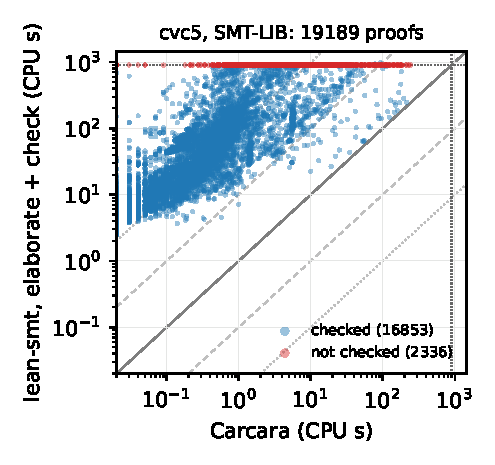
\includegraphics[width=0.49\textwidth]{carcara-vs-lean-smtlib-cvc5}
  \hfill
  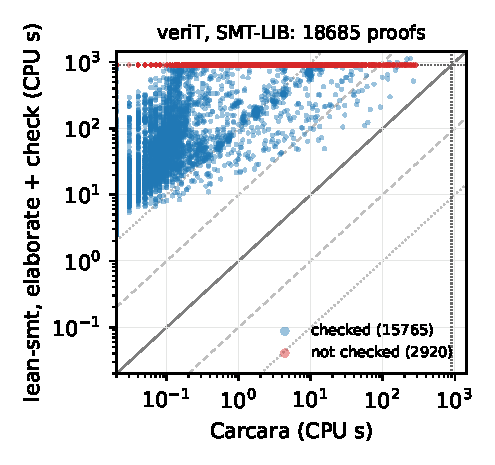
\includegraphics[width=0.49\textwidth]{carcara-vs-lean-smtlib-veriT}
  \caption{\carcara's check of the solver's proof against the elaboration plus
    \tactic's check, on the SMT-LIB proofs \carcara accepts, CPU seconds. Red
    points are proofs the checker did not finish within its limit; the grey
    lines are equality and factors of ten and a hundred.}
  \label{fig:smtlib}
\end{figure}

\paragraph{How the cost accumulates.} Figure~\ref{fig:cactus} plots, for each
configuration, the cumulative solving and checking time against the number of
benchmarks it validated, in the style of the \tactic paper. The checker
follows \carcara closely over the first thousands of benchmarks --- the small
proofs of the quantified logics, where both are dominated by the solving ---
and then separates in slope and in where it stops. Within the whole budget
\carcara needs for every proof it accepts, solving included (26.6 CPU hours
for \cvcv, 18.1 for \verit), the checker validates the first 13\,147 and
11\,982 of them.

\begin{figure}[t]
  \centering
  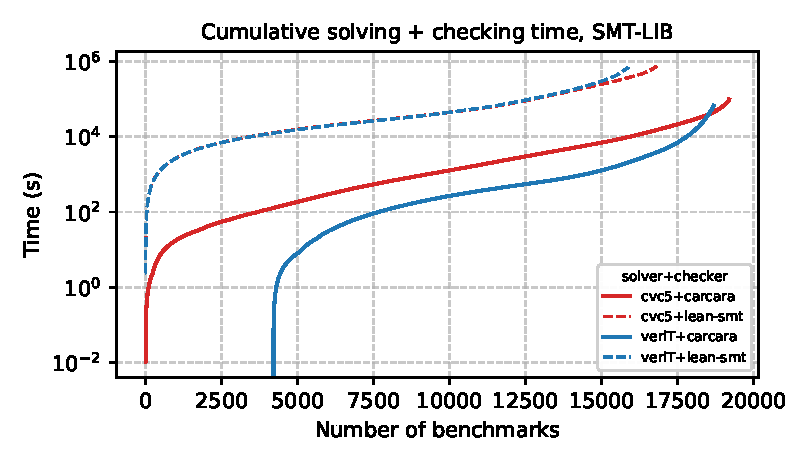
\includegraphics[width=0.72\textwidth]{cactus-smtlib}
  \caption{Cumulative solving and checking time against the number of SMT-LIB
    benchmarks whose proof the configuration validated. \carcara validates
    19\,188 \cvcv proofs in 26.6 CPU hours and 18\,683 \verit proofs in 18.1;
    the checker validates 16\,912 and 16\,098 in 184 and 171.}
  \label{fig:cactus}
\end{figure}

\paragraph{What is left.} Rule coverage is essentially complete and the
residue is small enough to enumerate. \cvcv leaves 2 proofs with a trusted
step, 8 \rulename{resolution} steps between them and all of one shape: a
premise carries a doubly negated literal \texttt{(not (not p))}, and \cvcv,
whose SAT solver knows no difference between that literal and \texttt{p},
eliminates both against a single \texttt{(not p)} in one chain. \carcara's
checker admits the step, since it matches literals up to one negation added or
removed, but its elaborator cannot order the chain and keeps the step without
pivots; the checker then resolves one syntactic pivot per premise, leaves the
\texttt{(not (not p))} standing, and the computed clause has a literal the
stated one lacks. Both proofs are QF\_UF hardware benchmarks
(\texttt{2018-Goel-hwbench}) that exhausted the memory in the previous round,
so the hole is new only in that the proofs now get that far; the remedy is to
resolve modulo double negation, which is sound and local to the chain. \verit
leaves 17: 10 \rulename{lia\_generic}, \verit's oracle rule, closed by
\texttt{omega} when in its fragment and trusted otherwise, 6
\rulename{th\_resolution}, and one \rulename{resolution} step whose kernel
check hit the memory cap. The 32 \rulename{distinct\_elim} steps of the
previous round, over the large enumerations of the ESC/Java benchmarks, are
gone: every case that round left except \rulename{lia\_generic} had a fix and
a regression test --- \rulename{evaluate} over equalities between propositions,
where \texttt{=} on \texttt{Prop} has no computable decidability instance, is
rewritten to \texttt{↔} before evaluating; \rulename{distinct\_elim}'s pairwise
conversion, which embedded the whole conjunct list in each of $n^2$
projections, is proved by congruence on the conjunction; and the
\rulename{bool\_simplify} steps \carcara's core pass had left unreduced are
reduced (Section~\ref{sec:carcara}) --- and this round confirms them. The 15
errors are not the same phenomenon as the timeouts; Section~\ref{sec:revealed}
takes them apart. The rest is scale: the timeouts, whose remedy is the
reflective resolution checker described in the accompanying notes, not a rule.

\subsection{Where the Time Goes, Rule by Rule}
\label{sec:perrule}

The 178$\times$ and 436$\times$ of the previous section are whole-proof
figures, and they say nothing about which steps are expensive. Because the
round checks the \emph{elaborated} proof twice --- once with \carcara, once
with the checker --- the two can be compared step for step over the same
population. Figure~\ref{fig:rules} draws, for the rules that carry the most
total time, the distribution over benchmarks of the mean time per step of that
rule.

The two solvers are pooled: their per-rule distributions are close enough that
separating them says nothing the whole-proof figures did not already say.
The distributions are wide but the ordering is stable, and three things stand
out. First, the gap is not uniform: it runs from under 300$\times$ on
\rulename{rare\_rewrite} and \rulename{distinct\_elim}, where the checker
replays a rewrite it can name, to four orders of magnitude on the
small clausal rules --- 4\,500$\times$ on \rulename{or\_neg} and
4\,600$\times$ on \rulename{and} --- where \carcara compares two
arrays and the checker builds and kernel-checks a term. Those rules are cheap
per step for both, but they are the most numerous by an order of magnitude
(84\,M \rulename{cong} and 178\,M \rulename{resolution} steps in the round),
so the ratio there is what sets the whole-proof figure.

Second, one rule dominates the total: \rulename{resolution} is 59\% of the
checker's time, and \rulename{semilattice\_simp} a further 12\%. More than half
of the number is one rule, and no amount of work on the arithmetic or rewriting
rules moves it: the remedy for the timeouts is a reflective resolution checker.

\rulename{and} was of another kind, and the previous round's figure was what
made us look. Its median then was 8.6\,ms, \emph{above} \rulename{resolution}'s
5.2\,ms and higher than every rule in the figure but \rulename{poly\_simp},
30\,000$\times$ \carcara's, and the rule was 14\% of the checker's time --- the
highest per-step cost of any high-volume rule, on a rule whose whole content is
to name the $i$-th conjunct of a premise. That was an artefact of how the proof
term was built rather than anything the rule demands. The reconstruction sends an n-ary
\lstinline{and} to a right-nested $p_0 \wedge (p_1 \wedge \ldots)$, which is
\lstinline{andN} of the list of conjuncts only after $n$ unfoldings; projecting
the $i$-th conjunct \emph{through} that list therefore charged every step for
the whole conjunction --- an $n$-element \lstinline{List Prop} rebuilt per step,
a \lstinline{decide} of $i < n$ over it, $n$ unfoldings of \lstinline{andN} to
reconcile the premise's stated type, and $i$ reductions of
\lstinline{List.getElem}. Projecting structurally instead costs nothing to
reduce: the premise's type is \emph{already} headed by $\wedge$, so
\lstinline{And.right} applies with no unfolding at all, and the conjunct that
comes out is the very term the conclusion was built from, so the kernel's
remaining check is a pointer comparison --- the same thing \carcara does with
its hash-consed \lstinline{Arc::ptr_eq}, arrived at from the other side. The
same holds of \rulename{not\_or} and of the CNF axioms, where
\rulename{or\_pos} collapses to a single node. The lesson generalizes past
these rules: where the consumer's type already \emph{is} the connective, walk
it; do not manufacture a list and index it. In this round the rule's median is
1.3\,ms and its share of the checker's time 3\%; per step, over each solver's
whole round, \cvcv's \rulename{and} steps cost 0.8\,ms against 3.8 before and
\verit's 1.7 against 18.9.

Third, the structural AC rules that replaced \rulename{aci\_simp}
(Section~\ref{sec:carcara}) are cheap on both sides:
\rulename{semilattice\_simp} at a median of 4.4\,ms and \rulename{poly\_simp}
at 11\,ms for the checker, with ratios of 850$\times$ and 790$\times$, better
than the clausal rules they are glued to. Splitting \rulename{aci\_simp} into rules
with a normal form did not cost checking time.

\begin{figure}[t]
  \centering
  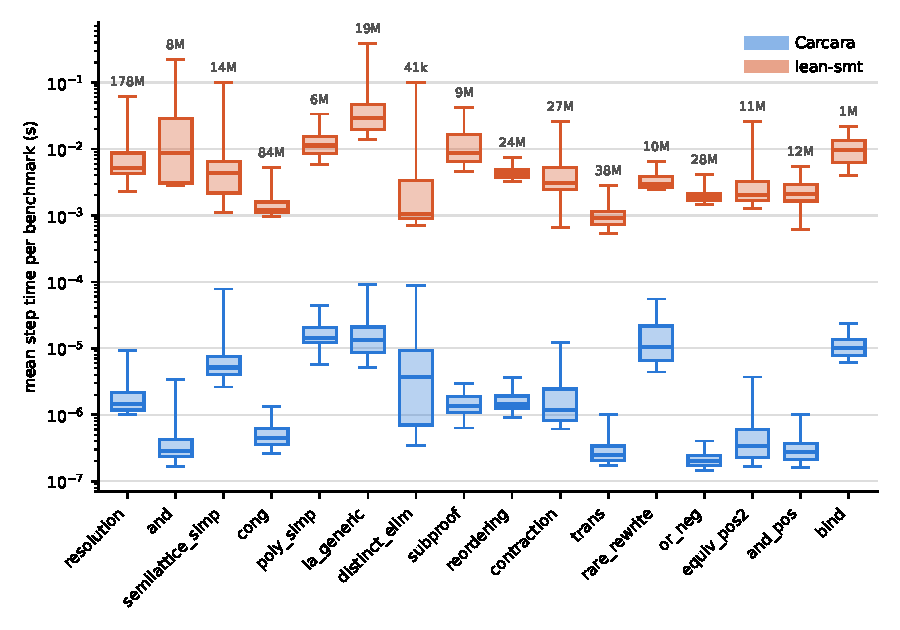
\includegraphics[width=\textwidth]{rule-boxplots}
  \caption{Mean time per step of each rule, over the benchmarks whose
    elaborated proof both checkers accept, for the sixteen rules with the
    largest total time, pooling the two solvers. The two series share an $x$
    position. Boxes are the quartiles and whiskers the 5th and 95th
    percentiles; the label above each group is the rule's total step count in
    the round. Note the log scale: \carcara sits
    three to four decades below \tactic throughout.}
  \label{fig:rules}
\end{figure}

\subsection{The Sledgehammer Set}
\label{sec:seventeen}

\paragraph{The corpus.} The 5\,000 SMT2 problems of the ``Seventeen provers
under the hammer'' baseline set, the quantified Isabelle goals the \tactic
paper evaluates on, with the same limits, and with \cvcv given the
instantiation options that paper used. These proofs are two to three orders
of magnitude smaller than the SMT-LIB ones: a median of 58 elaborated steps
for \cvcv and 110 for \verit, against tens of thousands in QF\_UF.

\paragraph{Outcomes.} Table~\ref{tab:seventeen} gives the round. Coverage is
close to total: the checker validates 2\,858 of the 2\,868 \cvcv proofs
\carcara accepts (99.7\%) and 2\,520 of the 2\,598 \verit ones (97.0\%), with
one and three timeouts and, for \verit, 21 runs that exhausted the memory.
What limits the round is the solver, not the checker --- 2\,869 and 2\,681 of
the 5\,000 problems are proved unsatisfiable at all --- and, for \verit,
\carcara's own check, which rejects 83 proofs, the integer/real parser
defect and \rulename{lia\_generic} steps. This corpus was last run before that
parser fix and the \rulename{ac\_simp} one; the SMT-LIB round above is the
current toolchain, and the \verit numbers here are correspondingly
pessimistic.

\begin{table}[t]
  \centering
  \caption{The Sledgehammer round, 5\,000 problems per solver; the columns of
    Table~\ref{tab:smtlib}, with the CPU hours each checker spends on the
    proofs it validates (elaboration included for \tactic) and the median
    slowdown on the proofs both validate.}
  \label{tab:seventeen}
  \small
  \begin{tabular}{l r r @{\quad} r r r r @{\quad} r r @{\quad} r}
    \toprule
    & & & \multicolumn{4}{c}{\tactic} & & & \\
    \cmidrule(lr){4-7}
    solver & proof & \carcara & valid & t/o & mem & holey & \carcara h & \tactic h & slower \\
    \midrule
    \cvcv  & 2\,869 & 2\,868 & 2\,858 & 1 &  0 &  9 & 0.04 & 4.5 & 234$\times$ \\
    \verit & 2\,681 & 2\,598 & 2\,520 & 3 & 21 & 51 & 0.02 & 3.8 & 483$\times$ \\
    \bottomrule
  \end{tabular}
\end{table}

\paragraph{Against \carcara.} Figure~\ref{fig:sh} is the comparison of
Figure~\ref{fig:smtlib} on this corpus. \carcara checks and elaborates in a
median of 0.02\,s and 0.01\,s; the checker's median of 5.0\,s (\cvcv) and
5.1\,s (\verit) is almost entirely the cost of loading the library, not of
checking, which is why the points form a horizontal band. On the 2\,843 and
2\,414 proofs both validate the checker is a median of 234$\times$ and
483$\times$ slower --- the same factors as in the SMT-LIB round, for a
different reason: there they measure a kernel replaying large derivations,
here a fixed startup cost against a checker that finishes in hundredths of a
second. Over the round the checker costs 4.5 and 3.8 CPU hours, against 72.2
and 92.8 hours of solving.
The few timeouts sit at the top of the size distribution --- 516 elaborated
steps for \cvcv's one, and 2\,876 to 3\,015 for \verit's three.

\begin{figure}[t]
  \centering
  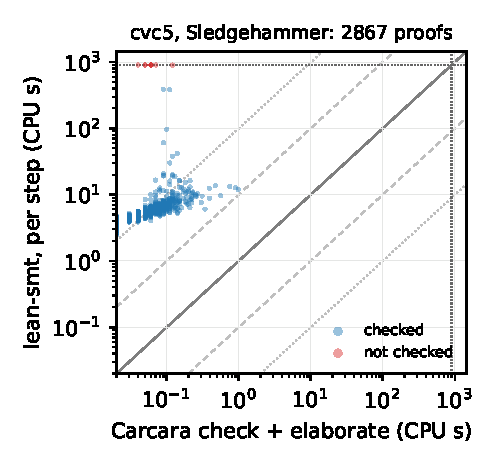
\includegraphics[width=0.49\textwidth]{carcara-vs-lean-seventeen-cvc5}
  \hfill
  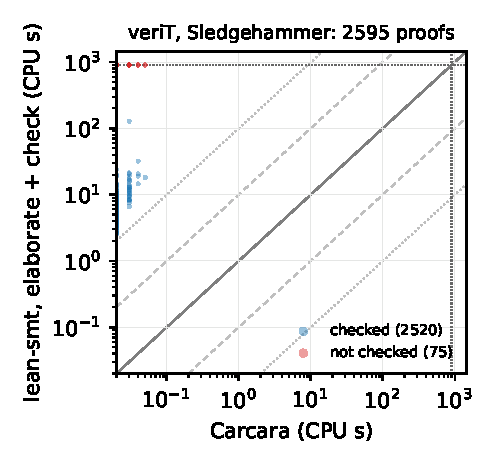
\includegraphics[width=0.49\textwidth]{carcara-vs-lean-seventeen-veriT}
  \caption{\carcara's check against the elaboration plus \tactic's check on
    the Sledgehammer proofs, CPU seconds. The band is the fixed cost of loading
    the library.}
  \label{fig:sh}
\end{figure}

\paragraph{How the cost accumulates.} Figure~\ref{fig:cactussh} is the
cumulative plot for this corpus, and it looks different in an instructive
way. Restricted to the proofs each configuration validates, solving is cheap
--- a median of a third of a second for \cvcv and a tenth for \verit --- so
the curves are dominated by what comes after it. \carcara disposes of all
2\,868 \cvcv proofs in 1.37 CPU hours including the solving, and of 2\,598
\verit ones in 1.22; the checker takes 5.8 and 5.0 for 2\,858 and 2\,520 of
them, four times as much for all but a handful fewer. The checker's curve is
close to a straight line, because on proofs this small its cost is the fixed
one of loading the library rather than anything about the derivation. Within
\carcara's whole budget the checker validates the first 1\,059 (\cvcv) and
963 (\verit).

\begin{figure}[t]
  \centering
  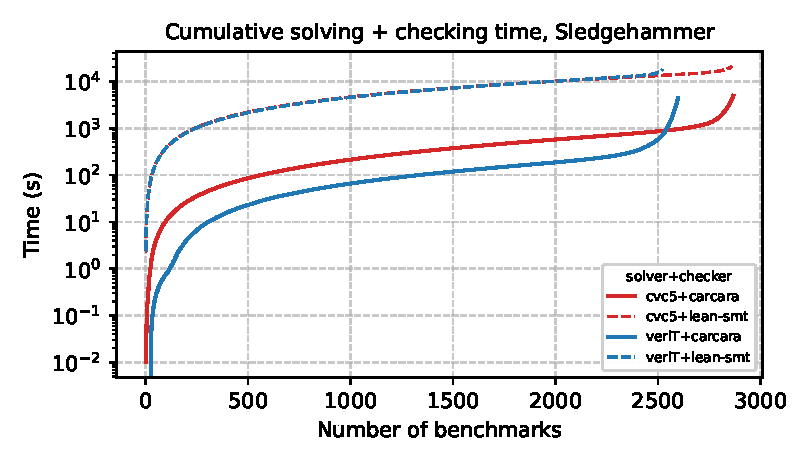
\includegraphics[width=0.72\textwidth]{cactus-seventeen}
  \caption{Cumulative solving and checking time against the number of
    Sledgehammer benchmarks whose proof the configuration validated. The
    \tactic curves are nearly straight.}
  \label{fig:cactussh}
\end{figure}

\paragraph{What is left.} The residue is small and, for each solver, of one
kind. \cvcv leaves nine proofs: eight whose \rulename{bind} step the kernel
rejected with a type mismatch --- \verit-style anchors that both keep a
variable and substitute it, since read consistently --- and one genuine
\rulename{hole}. \verit leaves 51, of which 47 are \rulename{onepoint}: 37
because the anchor assigned two or three variables at once where the
reconstructor supported one, and 13 because the guard equality sat in a body
shape its traversal did not reach; the reconstructor is now the general one,
following \carcara's \texttt{extract\_points}, and closes all of them. The
remaining four are three \rulename{qnt\_simplify} steps, since reconstructed,
and one \rulename{symm}/\rulename{trans} pair inside a \rulename{bind} whose
subproof both renames a variable and flips an equality; \carcara's
\rulename{symm} is name-syntactic there and the block has no consistent
reading as terms, so the remedy is on the producer's side --- the alpha-
equivalent \rulename{bind}s that \carcara's \texttt{polyeq} now closes by
\rulename{refl} remove every other instance of the pattern.

\subsection{What the Proofs Revealed}
\label{sec:revealed}

Checking against a second, independent reading of the rules paid off in both
directions. On the producer side: \verit's open named terms, its identity
substitutions \texttt{(:= (?x S) ?x)} in every \rulename{bind}, its fresh
names colliding with inner binders, the eleven Sledgehammer proofs whose
\rulename{bfun\_elim} the core pass silently kept, \carcara's modus-ponens
recipe, and the annihilator that \rulename{aci\_simp} did not name. On the
checker side: an \rulename{onepoint} guard refutation building
\lstinline{Or.inl} with an application builder that cannot infer the other
disjunct, exposed only when the cluster reached the \cvcv UF benchmarks; the
\texttt{Decidable} instance mismatch of Section~\ref{sec:rules}; the
quadratic construction of batch terms, caught by the first batch sweep; the
term-mode premise types; the hoisted definitional checks, which cost 49\,s on
a \rulename{trans} step whose links all matched syntactically; and the
polynomial normalizer's insertion fold, the per-literal tightening that gave
\texttt{omega} the whole local context, and the pairwise
\rulename{distinct\_elim} conversion, each a term whose size the kernel could
not bear. A rule-by-rule audit of the reconstructors against \carcara's
checkers, done after the SMT-LIB round, closed the remaining differences a
solver can produce --- the four argument orientations of \rulename{cong}
between two equalities, \rulename{distinct\_elim} over Booleans, both forms
of \rulename{la\_tautology}, the empty clause from \texttt{(not true)}, and
\rulename{lia\_generic} by \texttt{omega}. Every finding is a regression
test.

\paragraph{The failures the round leaves.} Beyond the timeouts, 15 \cvcv and
14 \verit runs end in an error. The previous round had 50 and 116, and they
were four distinct defects of the checker's front end rather than of any rule;
three were fixed between the rounds, and this round confirms the fixes.

\emph{Symbols with an apostrophe} (22 \cvcv and 27 \verit proofs, in UFLIA's
\texttt{tokeneer} and QF\_IDL's \texttt{sep}). \carcara's lexer admits
\texttt{'} inside a simple symbol so that the variables its
capture-avoiding substitutions rename (\texttt{x'}) round-trip, and its
printer decided what to quote with the same predicate. A symbol read from a
quoted \texttt{|status'|} was therefore printed back bare, which the SMT-LIB
grammar does not allow, so the elaborated proof was rejected by
\cvcv's parser --- the checker's own reader --- with \emph{Symbol `status' not
declared as a variable}. The printer now quotes any symbol containing an
apostrophe; quoting is always safe, since \texttt{|s|} and \texttt{s} denote
the same symbol. All 49 proofs now check.

\emph{Problems with more declarations than the interpreter's stack}
(5 \cvcv proofs, QF\_LIA's \texttt{SharedMemory} and \texttt{wireRouting}).
Lean's \texttt{withLocalDecls} nests one \texttt{withLocalDecl} per
declaration, so introducing the 160\,000 symbols and 280\,000 assertions of
those problems overflowed the interpreter's stack after minutes of work. A
flat variant that extends the local context in a loop and installs it once
checks the 15\,MB benchmark in 190\,s; four of the five now check, and the
fifth runs to the limit.

\emph{A resolution loop} (2 of the 8 \cvcv memory exhaustions). Alethe's
resolution removes \emph{every} occurrence of the pivot, so the chain
re-resolves while the working clause still holds it. Against a tautological
premise \texttt{(cl $l$ (not $l$))}, which \cvcv emits for
\rulename{not\_equiv2}-style splits, each pass erased the pivot and the
premise put it straight back: two million iterations before the memory cap.
The loop now stops when the premise contributes the pivot with the working
clause's own polarity. The remaining 6 had been taken for one step too large;
they were not, and all 8 now complete --- 6 valid, and the 2 with the trusted
\rulename{resolution} steps of Section~\ref{sec:smtlib}. Of \verit's 49, 34
now check and 13 remain, joined by one whose solver run had failed before,
all in QF\_IDL's \texttt{asp} and \texttt{parity} families and QF\_LIA's
\texttt{Dartagnan}.

\emph{An instance lookup that threw} (40 \verit proofs, 30 in QF\_UFIDL's
\texttt{pete2}, 8 in QF\_IDL's \texttt{RTCL}, 2 in \texttt{uclid}). The
reconstruction of an \texttt{ite} over propositions needs a
\texttt{Decidable} instance and searches for one before falling back to a
compositional classical instance. On these deeply nested ground chains over
integer differences the search threw its own \emph{failed to synthesize}
rather than reporting no instance, so the fallback never ran; and since this
happens while the problem's assertions are being reconstructed, before the
first step, it escaped the per-step guard that turns a failed reconstruction
into a trusted step and killed the run. A throw from the lookup is now a
fall-through. The 40 proofs, at a median of 61\,600 elaborated steps, belong
with the timeouts, and that is what they now are.

One group is not fixed. 15 \cvcv proofs, 13 of them in QF\_LIA's
\texttt{incrementalScheduling} and 2 in QF\_UFLIA, need higher-order reasoning
the checker does not have: \cvcv keeps a parameterised \texttt{define-fun} as an uninterpreted
symbol plus an assumption equating it to a \texttt{lambda}, rewrites inside
that lambda under a \rulename{bind}, and applies the result with
\rulename{ho\_cong}. The checker macro-expands definitions, so the unapplied
symbol means nothing to it, and it has no \rulename{ho\_cong}; these are the
only proofs in the round that use the rule. Supporting them means binding
\texttt{define-fun}s as functions rather than expanding them.

\section{Per-Step Against One-Term Submission}
\label{sec:shapes}

The per-step shape is the default, and the measurements above use it. This
section records what led to that choice: the comparison with the one-term
shape, in which the whole derivation is reconstructed as one term and checked
in a single kernel call --- the shape the \cpc path uses --- made on the
three-logic SMT-LIB round that preceded the twelve-logic one (QF\_UF, QF\_LIA
and QF\_LRA, 9\,812 benchmarks per solver) and on the Sledgehammer round. The
other variant of the default shape, \texttt{native}, is the subject of
Section~\ref{sec:native}.

\paragraph{SMT-LIB.} Figure~\ref{fig:stepshot} puts the two shapes side by
side. Per-step checking dominates in every logic and for both solvers: it
validates 1\,603 proofs (\cvcv) and 1\,644 (\verit) that the one-term shape
does not, and there is not a single proof in the other direction. On the
proofs both check it is also slightly cheaper. The one-term failures that are
not timeouts split in two. About six hundred per solver are the single kernel
call rejected for excessive memory, the cost of holding the whole derivation
at once. The other thousand per solver were a defect of term mode found by
this run: step by step, a premise is a hypothesis whose declared type is the
clause the proof states, while in one term it is the proof itself, whose
inferred type is only definitionally that clause, and the congruence
reconstructor, reading a premise's type, saw something else. A term-mode step
now carries its stated type; the memory failures remain, and the measurement
that led us to keep per-step checking as the default
(Section~\ref{sec:steps}) holds at corpus scale.

\begin{figure}[t]
  \centering
  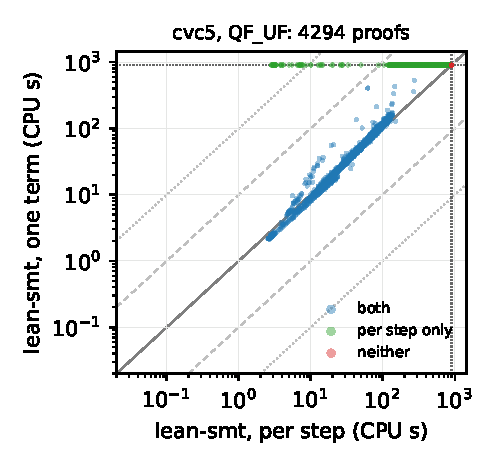
\includegraphics[width=0.49\textwidth]{step-vs-shot-QF_UF-cvc5}
  \hfill
  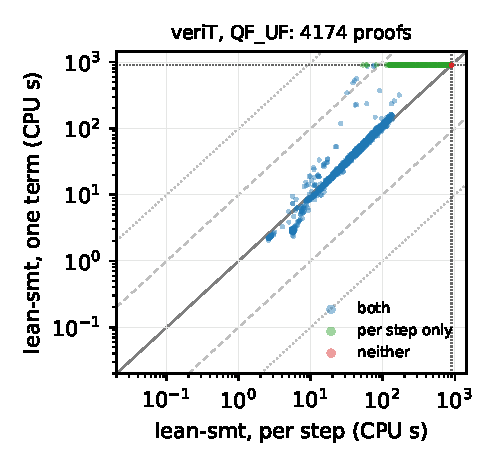
\includegraphics[width=0.49\textwidth]{step-vs-shot-QF_UF-veriT}
  \caption{The two kernel submission shapes on the same QF\_UF proofs, CPU
    seconds. A point on a dotted border is a proof the corresponding shape did
    not check; the grey lines are equality and factors of ten and a hundred.}
  \label{fig:stepshot}
\end{figure}

\begin{figure}[t]
  \centering
  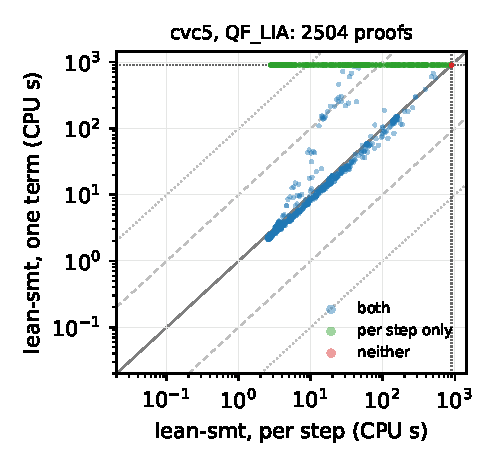
\includegraphics[width=0.49\textwidth]{step-vs-shot-QF_LIA-cvc5}
  \hfill
  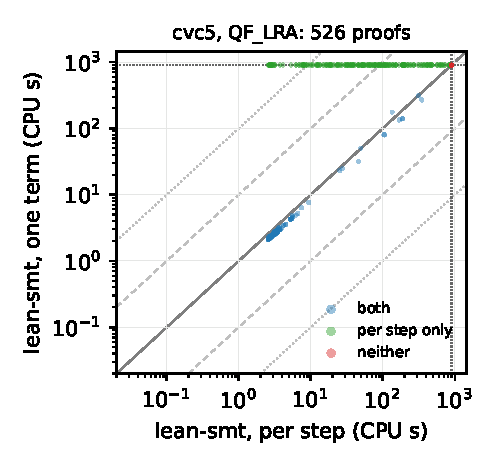
\includegraphics[width=0.49\textwidth]{step-vs-shot-QF_LRA-cvc5}
  \caption{The same comparison on \cvcv's arithmetic proofs, QF\_LIA (left) and
    QF\_LRA (right). The proofs are smaller, so both shapes reach further, and
    the one-term shape still loses 812 and 217 benchmarks.}
  \label{fig:stepshotarith}
\end{figure}

\paragraph{Sledgehammer.} On proofs this size the two shapes are nearly
indistinguishable --- 2\,725 against 2\,858 for \cvcv, 2\,508 against 2\,520
for \verit, at the same median cost (Figure~\ref{fig:stepshotsh}) --- which
is the other side of the SMT-LIB finding: the one-term shape loses only when
the derivation is too large to hold at once. Of the one-term failures, 133
(\cvcv) and 12 (\verit) were the term-mode premise-type defect, since fixed;
with it the two columns essentially coincide, and every remaining difference
is a proof the per-step arm also fails.

\begin{figure}[t]
  \centering
  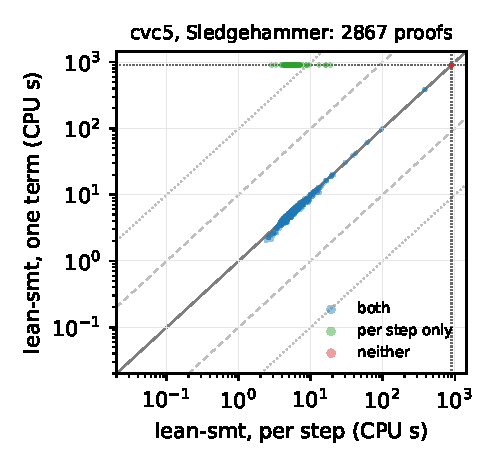
\includegraphics[width=0.49\textwidth]{step-vs-shot-seventeen-cvc5}
  \hfill
  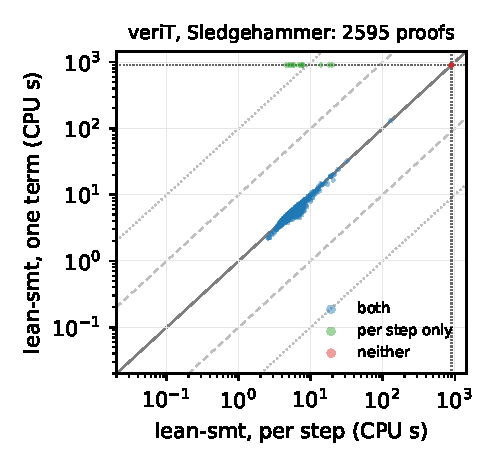
\includegraphics[width=0.49\textwidth]{step-vs-shot-seventeen-veriT}
  \caption{The two submission shapes on the Sledgehammer proofs, CPU seconds.
    The band along the diagonal is the fixed cost of loading the library.}
  \label{fig:stepshotsh}
\end{figure}

\clearpage
\section{The \texttt{native} Variant}
\label{sec:native}

The reconstructors have a second mode. Under \texttt{native}, the polynomial
normalizer behind the arithmetic rules and the decision procedure behind the
decidable side conditions --- the sign facts of \rulename{la\_generic}, the
nonzero coefficient of \rulename{poly\_simp\_rel}, and \rulename{evaluate}'s
ground equalities --- run
as compiled Lean code, and their verdicts enter the proof through
\texttt{nativeDecide} instead of being reduced by the kernel. It buys time and
costs trust: Lean's compiler and runtime join the kernel and \cvcv's parser in
the trusted base. Both sides are measured here on the twelve-logic SMT-LIB
round, where the two arms ran on the same node over the same elaborated proof,
under the same 900\,s limit and with the same per-step batching, so that every
benchmark is a matched pair.

\begin{table}[p]
  \centering
  \caption{The per-step shape against its \texttt{native} variant on the
    SMT-LIB round, over the benchmarks for which both arms ran: proofs
    validated with no trusted step and timeouts, per arm; then the paired
    verdicts --- validated by \emph{both} arms, by the plain arm only, by
    \texttt{native} only. The outcomes not shown are the same for both arms
    (0 and 14 memory failures, 2 and 17 proofs with a trusted step). The last column is the median ratio of \texttt{native}'s
    CPU time to the plain arm's, over the proofs both validate.}
  \label{tab:native}
  \small
  \setlength{\tabcolsep}{3.4pt}
  \begin{tabular}{l l r r @{\quad} r r @{\quad} r r r @{\quad} r}
    \toprule
    & & \multicolumn{2}{c}{per step} & \multicolumn{2}{c}{\texttt{native}}
      & \multicolumn{3}{c}{paired} & \\
    \cmidrule(lr){3-4} \cmidrule(lr){5-6} \cmidrule(lr){7-9}
    solver & logic & valid & t/o & valid & t/o & both & step & \texttt{nat.}
      & ratio \\
    \midrule
    \multirow{13}{*}{\cvcv}
      & QF\_UF    &   2\,524 &  1\,769 &   2\,524 &  1\,769 &   2\,522 &  2 &  2 & 0.993 \\
      & QF\_IDL   &      319 &     156 &      318 &     157 &      318 &  1 &  0 & 0.955 \\
      & QF\_RDL   &       38 &      35 &       41 &      32 &       38 &  0 &  3 & 0.838 \\
      & QF\_LIA   &   2\,337 &     158 &   2\,350 &     145 &   2\,337 &  0 & 13 & 0.841 \\
      & QF\_LRA   &      419 &     107 &      424 &     102 &      419 &  0 &  5 & 0.852 \\
      & QF\_UFIDL &       30 &       8 &       30 &       8 &       30 &  0 &  0 & 0.926 \\
      & QF\_UFLIA &      164 &       6 &      164 &       6 &      164 &  0 &  0 & 0.877 \\
      & QF\_UFLRA &      431 &      10 &      431 &      10 &      431 &  0 &  0 & 0.960 \\
      & UF        &   3\,154 &       1 &   3\,154 &       1 &   3\,154 &  0 &  0 & 0.922 \\
      & UFIDL     &       53 &       0 &       53 &       0 &       53 &  0 &  0 & 0.913 \\
      & UFLIA     &   7\,433 &       9 &   7\,432 &      10 &   7\,432 &  1 &  0 & 0.907 \\
      & UFLRA     &       10 &       0 &       10 &       0 &       10 &  0 &  0 & 0.873 \\
    \cmidrule(l){2-10}
      & total     &  16\,912 &  2\,259 &  16\,931 &  2\,240 &  16\,908 &  4 & 23 & 0.92 \\
    \midrule
    \multirow{13}{*}{\verit}
      & QF\_UF    &   2\,438 &  1\,736 &   2\,443 &  1\,731 &   2\,438 &  0 &  5 & 0.988 \\
      & QF\_IDL   &      213 &     316 &      217 &     312 &      212 &  1 &  5 & 0.978 \\
      & QF\_RDL   &       37 &      40 &       42 &      35 &       37 &  0 &  5 & 0.948 \\
      & QF\_LIA   &   2\,215 &     224 &   2\,215 &     224 &   2\,215 &  0 &  0 & 0.867 \\
      & QF\_LRA   &      421 &     155 &      426 &     150 &      421 &  0 &  5 & 0.865 \\
      & QF\_UFIDL &       67 &     197 &       67 &     197 &       67 &  0 &  0 & 0.988 \\
      & QF\_UFLIA &      172 &       1 &      172 &       1 &      172 &  0 &  0 & 0.952 \\
      & QF\_UFLRA &      357 &      58 &      357 &      58 &      357 &  0 &  0 & 1.003 \\
      & UF        &   2\,880 &       0 &   2\,880 &       0 &   2\,880 &  0 &  0 & 0.902 \\
      & UFIDL     &       51 &       0 &       51 &       0 &       51 &  0 &  0 & 0.918 \\
      & UFLIA     &   7\,237 &       2 &   7\,237 &       2 &   7\,237 &  0 &  0 & 0.922 \\
      & UFLRA     &       10 &       0 &       10 &       0 &       10 &  0 &  0 & 0.968 \\
    \cmidrule(l){2-10}
      & total     &  16\,098 &  2\,729 &  16\,117 &  2\,710 &  16\,097 &  1 & 20 & 0.92 \\
    \bottomrule
  \end{tabular}
\end{table}

\paragraph{Outcomes.} Table~\ref{tab:native} gives the round per logic.
\texttt{native} validates 19 more \cvcv proofs (16\,931 against 16\,912) and
19 more \verit ones (16\,117 against 16\,098), a tenth of a percent of either
population, and what gain there is is timeouts avoided: 2\,259 fall to
2\,240 and 2\,729 to 2\,710. Nothing else moves. The memory failures are the
same 0 and 14 runs, the proofs with a trusted step the same 2 and 17, and no
proof's trusted-step count differs between the arms.

\paragraph{Paired.} Figure~\ref{fig:native} puts the two arms on the same
proof. Per logic the two columns of validated proofs are equal or differ by a
handful, and the paired counts say why: 16\,908 (\cvcv) and 16\,097 (\verit)
proofs are validated by both arms, 23 and 20 by \texttt{native} only, 4 and 1
by the plain arm only. Both asymmetries sit against the limit: every proof
either arm wins alone is one the other left running at the 900\,s mark. What
separates the arms is how close a proof already was to the timeout, not what
either can check.

\begin{figure}[t]
  \centering
  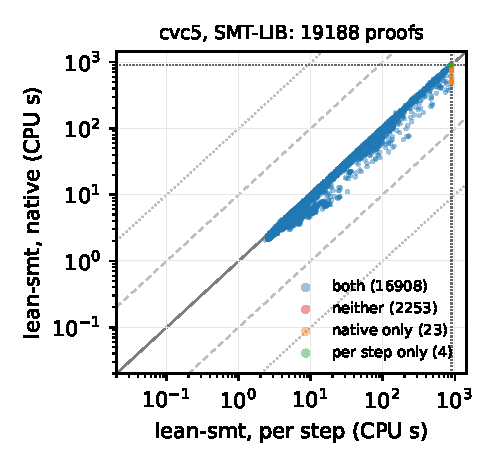
\includegraphics[width=0.49\textwidth]{step-vs-native-cvc5}
  \hfill
  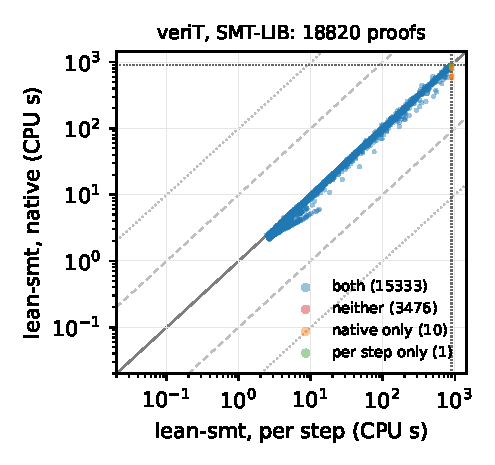
\includegraphics[width=0.49\textwidth]{step-vs-native-veriT}
  \caption{The per-step shape against its \texttt{native} variant on the same
    SMT-LIB proofs, CPU seconds. A point on a dotted border is a proof the
    corresponding arm did not validate; the grey lines are equality and
    factors of ten and a hundred. The cloud sits just below the diagonal, and
    the points either arm loses alone are all against the limit.}
  \label{fig:native}
\end{figure}

\paragraph{Where the time goes.} On the proofs both arms validate,
\texttt{native} is faster on 92.5\% (\cvcv) and 92.3\% (\verit) of them, and
the median ratio of its CPU time to the plain arm's is 0.92 for both solvers,
with the middle half of the proofs between 0.87 and 0.97. Summed, 172.8 CPU
hours become 164.2 and 165.2 become 161.4. Figure~\ref{fig:nativekernel}
isolates the kernel's share of that: its median falls from 606 to 409\,ms per
\cvcv proof and from 573 to 491\,ms per \verit one, 106.7 CPU hours to 95.2
and 109.4 to 105.3, but it still accounts for 58\% and 65\% of each arm's time
against 62\% and 66\% before. The saving is a slice of the kernel's work rather than most of it,
because what the kernel spends its time on is the resolution chains and the
congruences, which \texttt{native} does not touch. The per-logic medians of
the last column of Table~\ref{tab:native} locate the gain exactly: 0.84 to
0.85 in \cvcv's QF\_LIA, QF\_LRA and QF\_RDL, where the normalizer runs on
every arithmetic step, against 0.993 and 0.988 in QF\_UF, where it never runs
at all.

\begin{figure}[!tb]
  \centering
  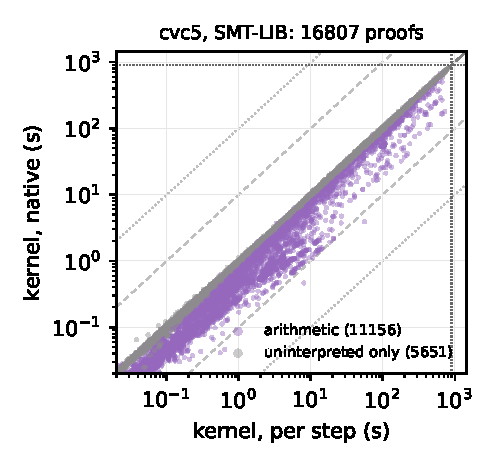
\includegraphics[width=0.49\textwidth]{kernel-step-vs-native-cvc5}
  \hfill
  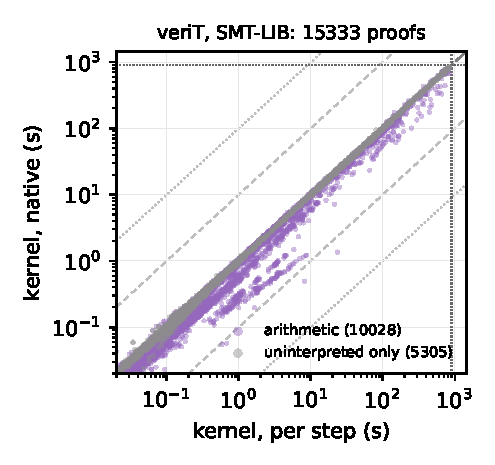
\includegraphics[width=0.49\textwidth]{kernel-step-vs-native-veriT}
  \caption{The kernel's own time in the two arms, on the proofs both validate,
    seconds; the proofs of a logic with arithmetic are drawn apart from those
    of QF\_UF and UF. The saving is where the normalizer runs: the
    uninterpreted proofs lie on the diagonal, the arithmetic ones below it.}
  \label{fig:nativekernel}
\end{figure}

\paragraph{What it is worth.} The variant changes nothing about what is
admitted without proof: over the 33\,005 matched pairs both arms validate, the
number of trusted steps is identical on every single one, and the holey
population is the same. So \texttt{native} buys 8\% of the median checking
time and a tenth of a percent of the corpus, at the price of the compiler and
the runtime in the trusted base. That is the wrong trade for a checker whose
point is the kernel, and the plain per-step shape stays the default; the
variant is kept for the one case its numbers do favour, a large arithmetic
proof that will not check in the time available otherwise.

\begin{thebibliography}{1}
\bibitem{Barbosa2020}
Barbosa, H., Blanchette, J.C., Fleury, M., Fontaine, P.: Scalable fine-grained
proofs for formula processing. Journal of Automated Reasoning 64(3), 485--510
(2020)
\bibitem{Mohamed2025}
Mohamed, A., Mascarenhas, T., Khan, H., Barbosa, H., Reynolds, A., Qian, Y.,
Tinelli, C., Barrett, C.: Lean-SMT: An SMT tactic for discharging proof goals in
Lean. In: CAV 2025
\bibitem{Andreotti2023}
Andreotti, B., Lachnitt, H., Barbosa, H.: Carcara: An efficient proof checker
and elaborator for SMT proofs in the Alethe format. In: TACAS 2023
\end{thebibliography}

\end{document}

%%% Local Variables:
%%% mode: LaTeX
%%% TeX-master: t
%%% End:
